% HITA 2026 poster — "Engagement Scoring and Status Segmentation of eBook
% Subscribers using Exploratory Data Analysis"
% Frame: Unofficial University of Cambridge Poster Template
% https://github.com/andiac/gemini-cam (fork of gemini)
%
% SIZE: 3 ft x 2 ft portrait = 91.44 cm x 60.96 cm.
% All template font sizes and fixed lengths are the 84 x 118 cm values x 0.725.

% Beamer loads xcolor itself, so the 'table' option must be passed
% before the document class to avoid an option clash (both locally and in Overleaf).
\PassOptionsToPackage{table}{xcolor}
\documentclass[final]{beamer}
% ====================
% Packages
% ====================

% \usepackage[T1]{fontenc}
% \usepackage{lmodern}

% ====================
% Fonts
% ====================
\usepackage{fontspec}
\usefonttheme{professionalfonts}
\setmainfont{TeX Gyre Heros}
\renewcommand{\familydefault}{\sfdefault}

\setbeamerfont{normal text}{family=\sffamily}
\setbeamerfont{block title}{family=\sffamily,series=\bfseries}
\setbeamerfont{block body}{family=\sffamily}
\setbeamerfont{headline}{family=\sffamily,series=\bfseries}
\setbeamerfont{footline}{family=\sffamily}
\setbeamerfont{caption}{family=\sffamily}

\usepackage[orientation=portrait,size=custom,width=60.96,height=91.44,scale=1.0]{beamerposter}
% beamerposter sets \normalsize to 24.88 pt at scale=1.0; the brief requires
% 20 pt body, so restore it after the package has redefined the size ladder.
\renewcommand{\normalsize}{\fontsize{20}{25}\selectfont}
\usepackage{multicol}
\usetheme{gemini}

% No visible link boxes in the printed PDF
\hypersetup{hidelinks}

%=======================
% FONT SETTINGS  (84x118 values x 0.725: 68/34/28/40/28/22)
%=======================
% Poster Title
\setbeamerfont{title}{
    family=\sffamily,
    series=\bfseries,
    size=\fontsize{49}{55}\selectfont
}
% Authors
\setbeamerfont{author}{
    family=\sffamily,
    size=\fontsize{25}{29}\selectfont
}
% Affiliations
\setbeamerfont{institute}{
    family=\sffamily,
    size=\fontsize{20}{25}\selectfont
}
% Section Headings
\setbeamerfont{block title}{
    family=\sffamily,
    series=\bfseries,
    size=\fontsize{29}{33}\selectfont
}
% Highlighted Section Headings
\setbeamerfont{block title alerted}{
    family=\sffamily,
    series=\bfseries,
    size=\fontsize{29}{33}\selectfont
}
% Body Text
\setbeamerfont{normal text}{
    family=\sffamily,
    size=\fontsize{20}{25}\selectfont
}
% Figure/Table Captions
\setbeamerfont{caption}{
    family=\sffamily,
    size=\fontsize{16}{19}\selectfont
}

\usecolortheme{nott}
\usepackage{graphicx}
\usepackage{booktabs}
\usepackage{tikz}
\usetikzlibrary{arrows.meta, positioning}
\usepackage{pgfplots}
\pgfplotsset{compat=1.14}
\usepackage{anyfontsize}
\usepackage{xcolor}
\usepackage{caption}

% ====================
% Lengths
% ====================
% If you have N columns, choose \sepwidth and \colwidth such that
% (N+1)*\sepwidth + N*\colwidth = \paperwidth
\newlength{\sepwidth}
\newlength{\colwidth}
\setlength{\sepwidth}{0.025\paperwidth}
\setlength{\colwidth}{0.45\paperwidth}
\newcommand{\separatorcolumn}{\begin{column}{\sepwidth}\end{column}}

% ====================
% Title
% ====================

\title{Engagement Scoring and Status \\ Segmentation of eBook Subscribers \\ using Exploratory Data Analysis}

\author{Tridha Mitra* \quad Kasturi Kathare \quad Vidushi Barnwal \quad Ayana Deb \quad Krisha Kadam}

\institute[shortinst]{
\itshape
Presented at HITA 2026, International Conference on Hybrid Intelligence: Theories and Applications,\\
School of Technology Management \& Engineering,
Navi-Mumbai, India, October 30--31, 2026.
}

% ====================
% Footer (optional)
% ====================
\footercontent{
  \href{}{}
  \hfill
  HITA 2026, STME Navi-Mumbai, India, October 30--31, 2026 \hfill
  \href{}{E-mail ID: (to be added)}
% (can be left out to remove footer)
}


% ====================
% Logo (optional)
% ====================

% use this to include logos on the left and/or right side of the header
% (heights are the 10.8 / 10.0 cm values x 0.725):
\logoright{
\includegraphics[height=7.8cm]{logos/HITA_2026.png}}
\logoleft{
\includegraphics[height=7.25cm]{logos/NMIMS Logo.png}}

% The gemini headline pads with 5ex/3ex/5ex, which at a 49 pt title is ~15 cm
% of vertical space on a 91 cm page. Same design, compact spacing for the
% 3 ft x 2 ft format: navy band, logos left/right, centred title block, rule.
\setbeamertemplate{headline}{
  \begin{beamercolorbox}{headline}
    \vskip1.2ex
    \hbox to \paperwidth{%
      \hspace*{1.1cm}%
      \begin{minipage}[c]{0.15\paperwidth}\raggedright
        \ifdefined\insertlogoleft\insertlogoleft\fi
      \end{minipage}\hfill
      \begin{minipage}[c]{0.65\paperwidth}\centering
        {\usebeamerfont{title}\usebeamercolor[fg]{headline title}\inserttitle\par}
        \vspace{0.30cm}
        {\usebeamerfont{author}\usebeamercolor[fg]{headline author}\insertauthor\par}
        \vspace{0.22cm}
        {\usebeamerfont{institute}\usebeamercolor[fg]{headline institute}\insertinstitute\par}
      \end{minipage}\hfill
      \begin{minipage}[c]{0.15\paperwidth}\raggedleft
        \ifdefined\insertlogoright\insertlogoright\fi
      \end{minipage}%
      \hspace*{1.1cm}%
    }
    \vskip1.2ex
    \begin{beamercolorbox}[wd=\paperwidth,colsep=0.35ex]{headline rule}\end{beamercolorbox}
  \end{beamercolorbox}
}

% ====================
% Body
% ====================

\begin{document}

\begin{frame}[t]
\begin{columns}[t]
\separatorcolumn

\begin{column}{\colwidth}

% ---------- 1. Problem Statement ----------
\begin{block}{\textbf{Problem Statement}}
Digital subscription platforms run on \textbf{recurring revenue}: keeping a subscriber costs less than acquiring a new one, yet platforms treat every subscriber alike and cannot tell who is staying from who is leaving, so \textbf{generic retention campaigns} miss the readers they should reach. \textbf{Research question:} which behavioural and demographic signals distinguish high-engagement from low-engagement eBook subscribers, and what should the platform do about each group? \textbf{Phase 1} (customer file, 16,404 customers) measured subscription propensity (33.2\% subscribers); \textbf{Phase 2} (engagement file, 5,455 subscribers) builds the score and the Active / Inactive / Churned status.
\end{block}
\vspace{0.5cm}

% ---------- 2. Literature Review ----------
\begin{block}{\textbf{Literature Review}}
\fontsize{20}{25}\selectfont
\centering
\setlength{\tabcolsep}{4pt}
\begin{tabular}{p{0.17\linewidth} p{0.30\linewidth} p{0.19\linewidth} p{0.28\linewidth}}
\toprule
\textbf{Theme} & \textbf{What research shows} & \textbf{Source} & \textbf{How we used it} \\
\midrule
Engagement drivers & Motivated readers show fewer, longer sessions; session depth marks engagement & Vuorinen \cite{vuorinen2024} & Session minutes in the score (weight 0.25) \\
Churn signals & Declining usage and fast content depletion precede cancellation & Bolton \cite{bolton1999}; Godinho \cite{godinho2020} & Recency (0.40) and logins (0.35); status rules \\
Subscriber segmentation & Churn drivers differ by segment; a risk score alone mis-targets offers & Rani \cite{rani2023}; Ascarza \cite{ascarza2018} & Active / Inactive / Churned; Low / Medium / High tiers \\
EDA for churn analysis & Exploration and variable selection expose the churn signal before modelling & Coussement \cite{coussement2008} & $r = 0.88$ check; books kept out of the score \\
Personalisation \& retention & Personalised recommendations lift retention; timed win-back beats flat discounting & Gomez-Uribe \cite{gomezuribe2016}; Thomas \cite{thomas2004} & One action per status in Recommendations \\
\bottomrule
\end{tabular}
\end{block}
\vspace{0.5cm}

% ---------- 3. Dataset ----------
\begin{block}{\textbf{Dataset}}
\fontsize{20}{25}\selectfont
\centering
\setlength{\tabcolsep}{4pt}
\begin{tabular}{p{0.28\linewidth} p{0.17\linewidth} p{0.49\linewidth}}
\toprule
\textbf{File} & \textbf{Rows after cleaning} & \textbf{Key fields} \\
\midrule
customer\_data.csv & 16,404 customers & demographics, income, monthly spend, subscriber flag \\
eBook\_Engagement.csv & 5,455 subscribers & logins, session minutes, books accessed, days since last activity, genre, tenure \\
\bottomrule
\end{tabular}

\raggedright
\vspace{0.3em}
\textbf{Synthetic data}; the two files join on Customer ID (5,455 of 5,455 matched).
\end{block}
\vspace{0.5cm}

% ---------- 4. Cleaning & Preprocessing ----------
\begin{block}{\textbf{Cleaning \& Preprocessing}}
\fontsize{20}{25}\selectfont
\centering
\setlength{\tabcolsep}{4pt}
\begin{tabular}{p{0.44\linewidth} p{0.36\linewidth} p{0.14\linewidth}}
\toprule
\textbf{Issue found} & \textbf{Action} & \textbf{Count} \\
\midrule
Duplicate customer IDs & dropped, keep-first & 115 \\
Duplicate engagement rows & dropped & 45 \\
Two-digit birth years & century added, age computed & 16,519 \\
Genre spelling variants & mapped to 8 genres & 26 \\
Negative days since activity & set to missing & 6 \\
Logins $>$ 60, sessions $>$ 180 min, books $>$ 60 & set to missing (decimal shift) & 7 / 8 / 7 \\
Recency $>$ 365 days & kept as-is (capture cap) & 11 \\
Blank logins, sessions, books & median-filled & 144 \\
Missing or invalid recency & never imputed, left Unclassified & 33 \\
Names and street addresses & dropped, no analytic use & 2 fields \\
\bottomrule
\end{tabular}
\end{block}
\vspace{0.5cm}

% ---------- 5. Analysis ----------
\begin{block}{\textbf{Analysis}}
\begin{itemize}
\justifying
\item \textbf{Score:} $100 \times (0.40R + 0.35L + 0.25S)$ on min--max scaled inputs, with $R$ = inverted recency, $L$ = logins, $S$ = session minutes. \textbf{One reason per weight:} recency 0.40 is the most direct signal of leaving, logins 0.35 measure usage frequency, session minutes 0.25 measure depth of use.
\item \textbf{Books Accessed excluded:} $r = 0.88$ with logins, so including it would double-count usage. Terciles at 40.80 and 51.25 give Low / Medium / High.
\item \textbf{Status rules} (written and approved before computing): Active $\le$ 30 days since last activity \emph{and} $\ge$ 1 login/month; Inactive 31--90 days; Churned $>$ 90 days.
\end{itemize}

\begin{center}
\begin{tikzpicture}[
  flow/.style={draw=nottblue, line width=1.2pt, rounded corners=6pt,
               fill=nottblue, text=white, minimum height=1.85cm,
               text width=14.5cm, align=center, inner sep=6pt,
               font=\bfseries\fontsize{20}{25}\selectfont},
  flowalt/.style={flow, fill=white, text=nottblue},
  link/.style={-{Stealth[length=5mm]}, line width=1.7pt, draw=nottblue}
]
\node[flow]    (files) {Two raw files};
\node[flowalt, below=1.15cm of files]  (clean) {Clean, join, EDA};
\node[flow,    below=1.15cm of clean]  (score) {Engagement score 0--100};
\node[flowalt, below=1.15cm of score]  (status) {Status rules};
\node[flow,    below=1.15cm of status] (recs)  {Recommendations};
\draw[link] (files.south)  -- (clean.north);
\draw[link] (clean.south)  -- (score.north);
\draw[link] (score.south)  -- (status.north);
\draw[link] (status.south) -- (recs.north);
\end{tikzpicture}
\end{center}

\vspace{-0.6em}
\captionof{figure}{End-to-end pipeline: two raw files become a cleaned, joined, scored and status-labelled subscriber base.}
\label{fig:pipeline}
\end{block}

\end{column}

\separatorcolumn

\begin{column}{\colwidth}

% ---------- 6. Charts ----------
\begin{block}{\textbf{Charts}}

\begin{center}
\begin{minipage}[t]{0.38\linewidth}
    \centering
    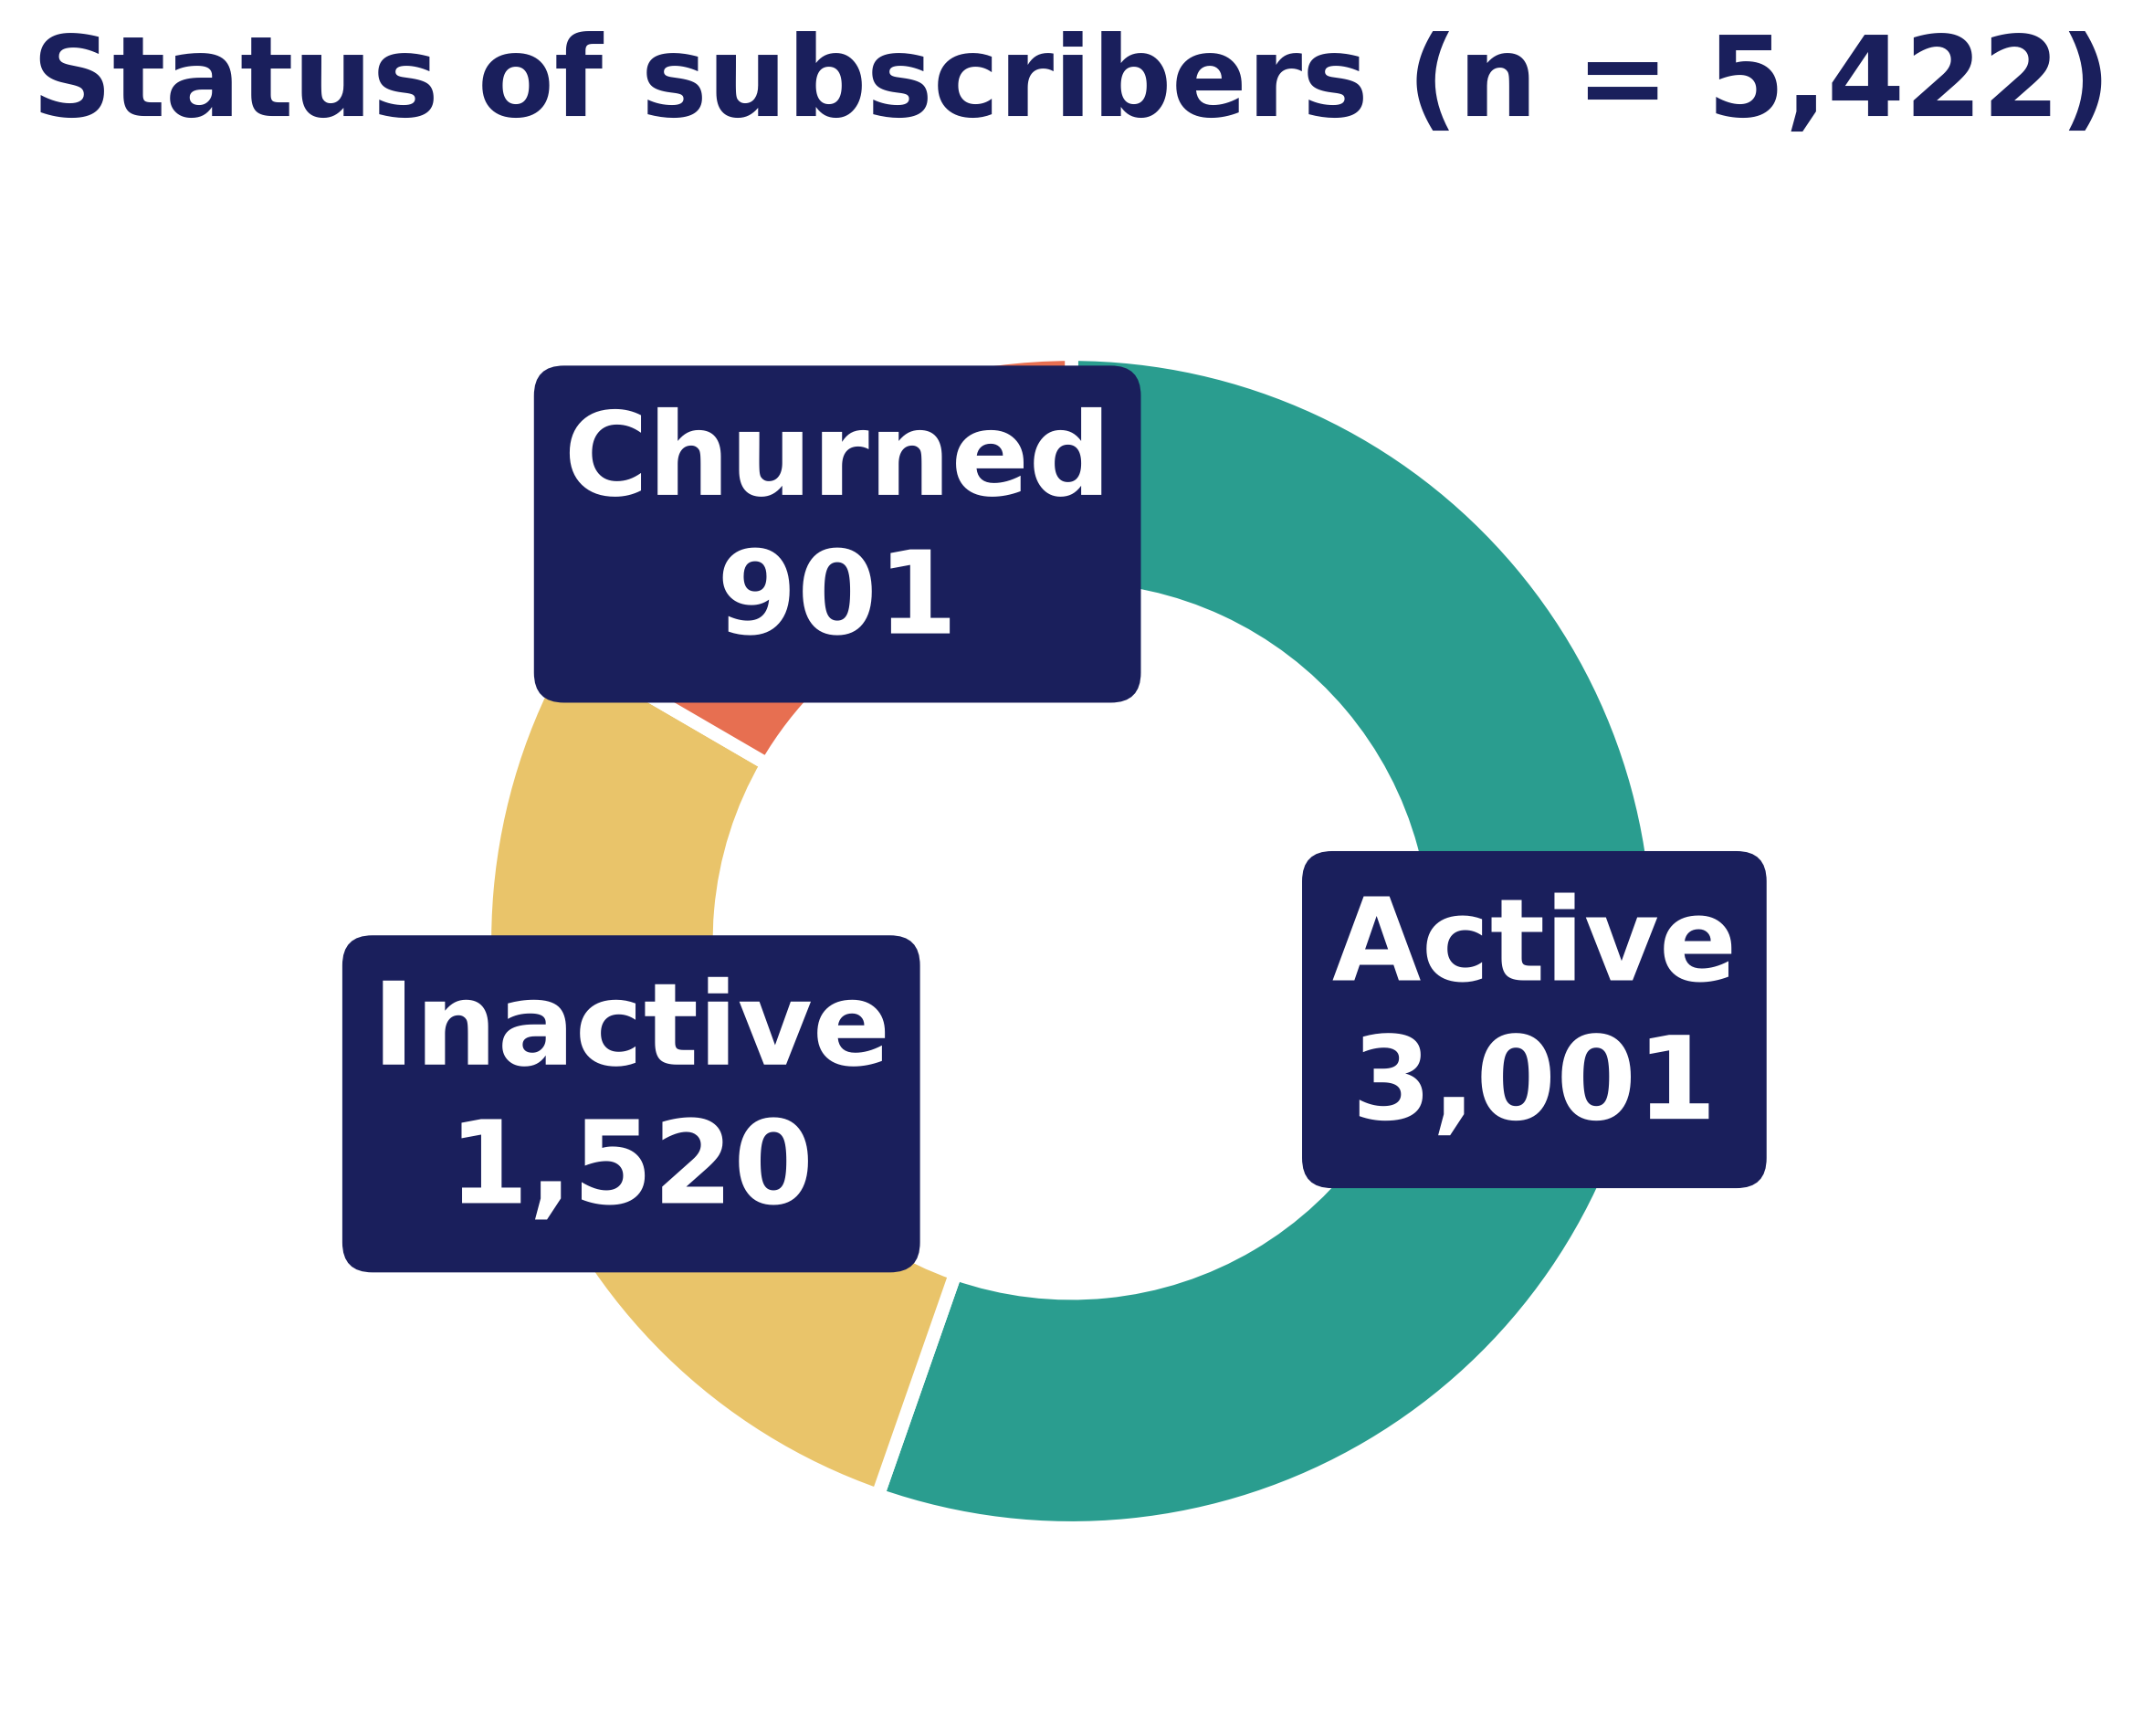
\includegraphics[width=\linewidth]{figures/f1_status_doughnut.png}
    \captionof{figure}{55.3\% Active, 28.0\% Inactive, 16.6\% Churned (33 unclassified).}
\end{minipage}\hfill
\begin{minipage}[t]{0.38\linewidth}
    \centering
    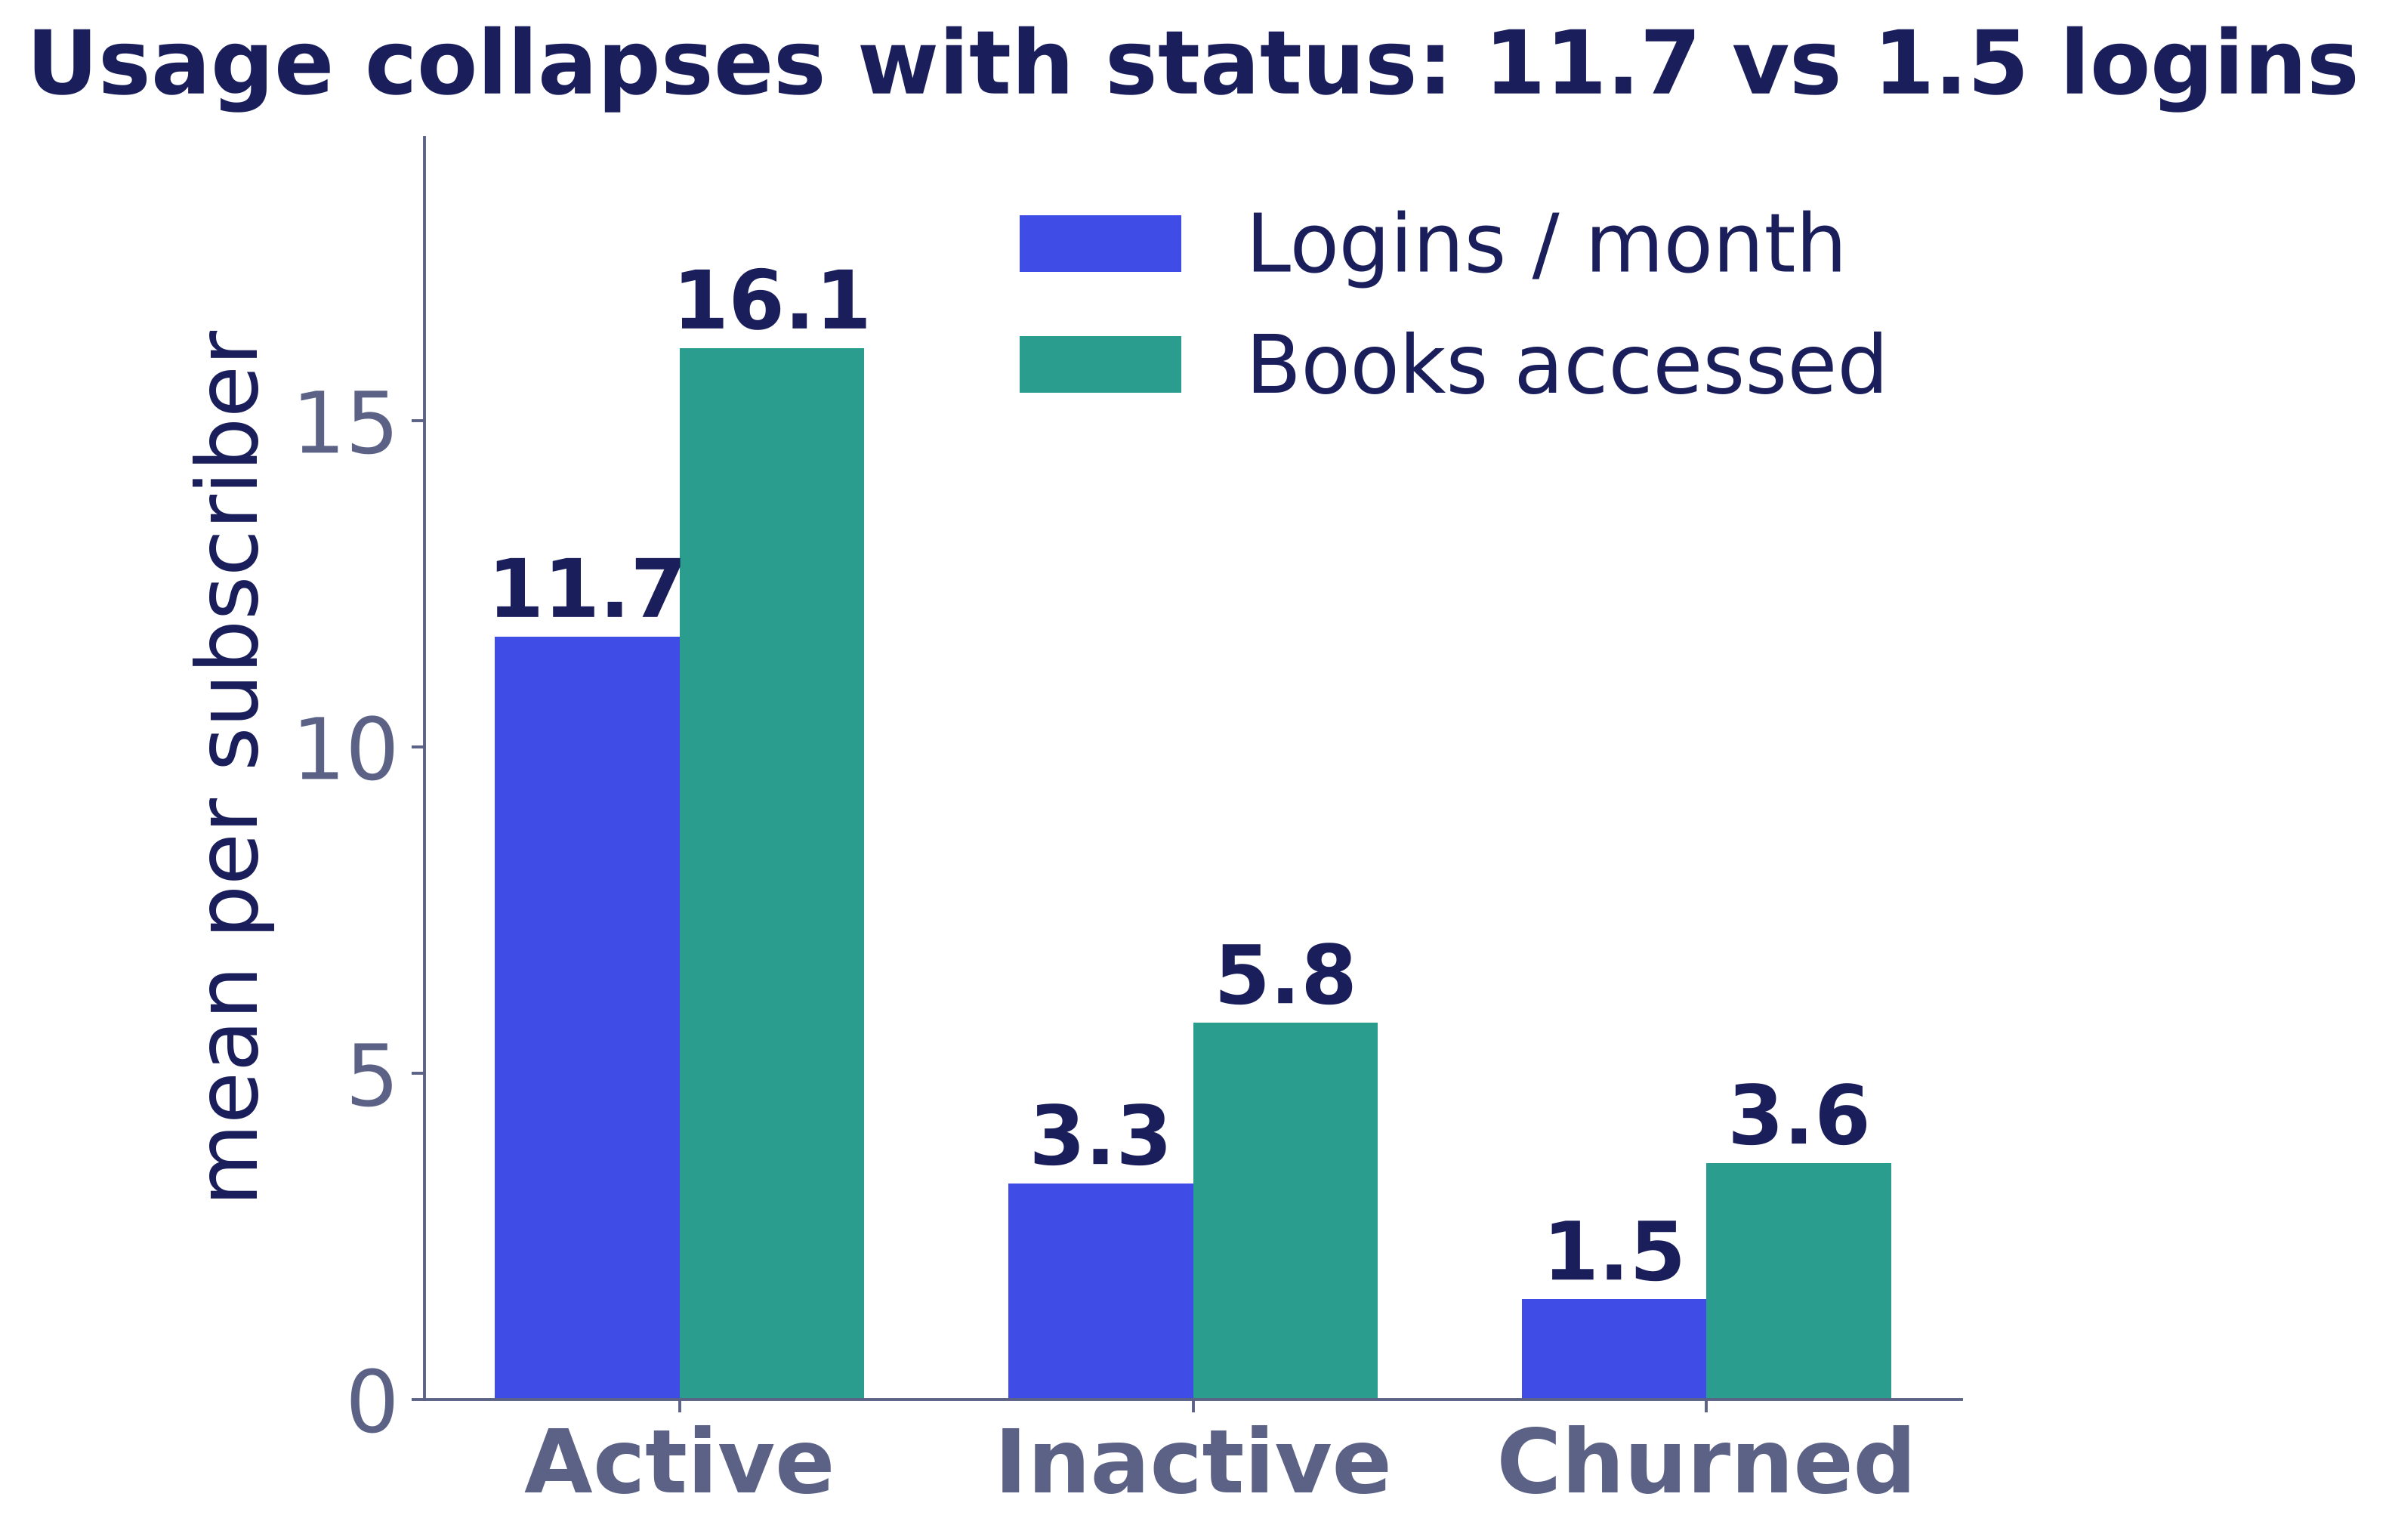
\includegraphics[width=\linewidth]{figures/f4_logins_books_by_status.png}
    \captionof{figure}{Churned log in 1.5 times a month vs 11.7 for Active.}
\end{minipage}
\end{center}

\vspace{0.4em}
\centering
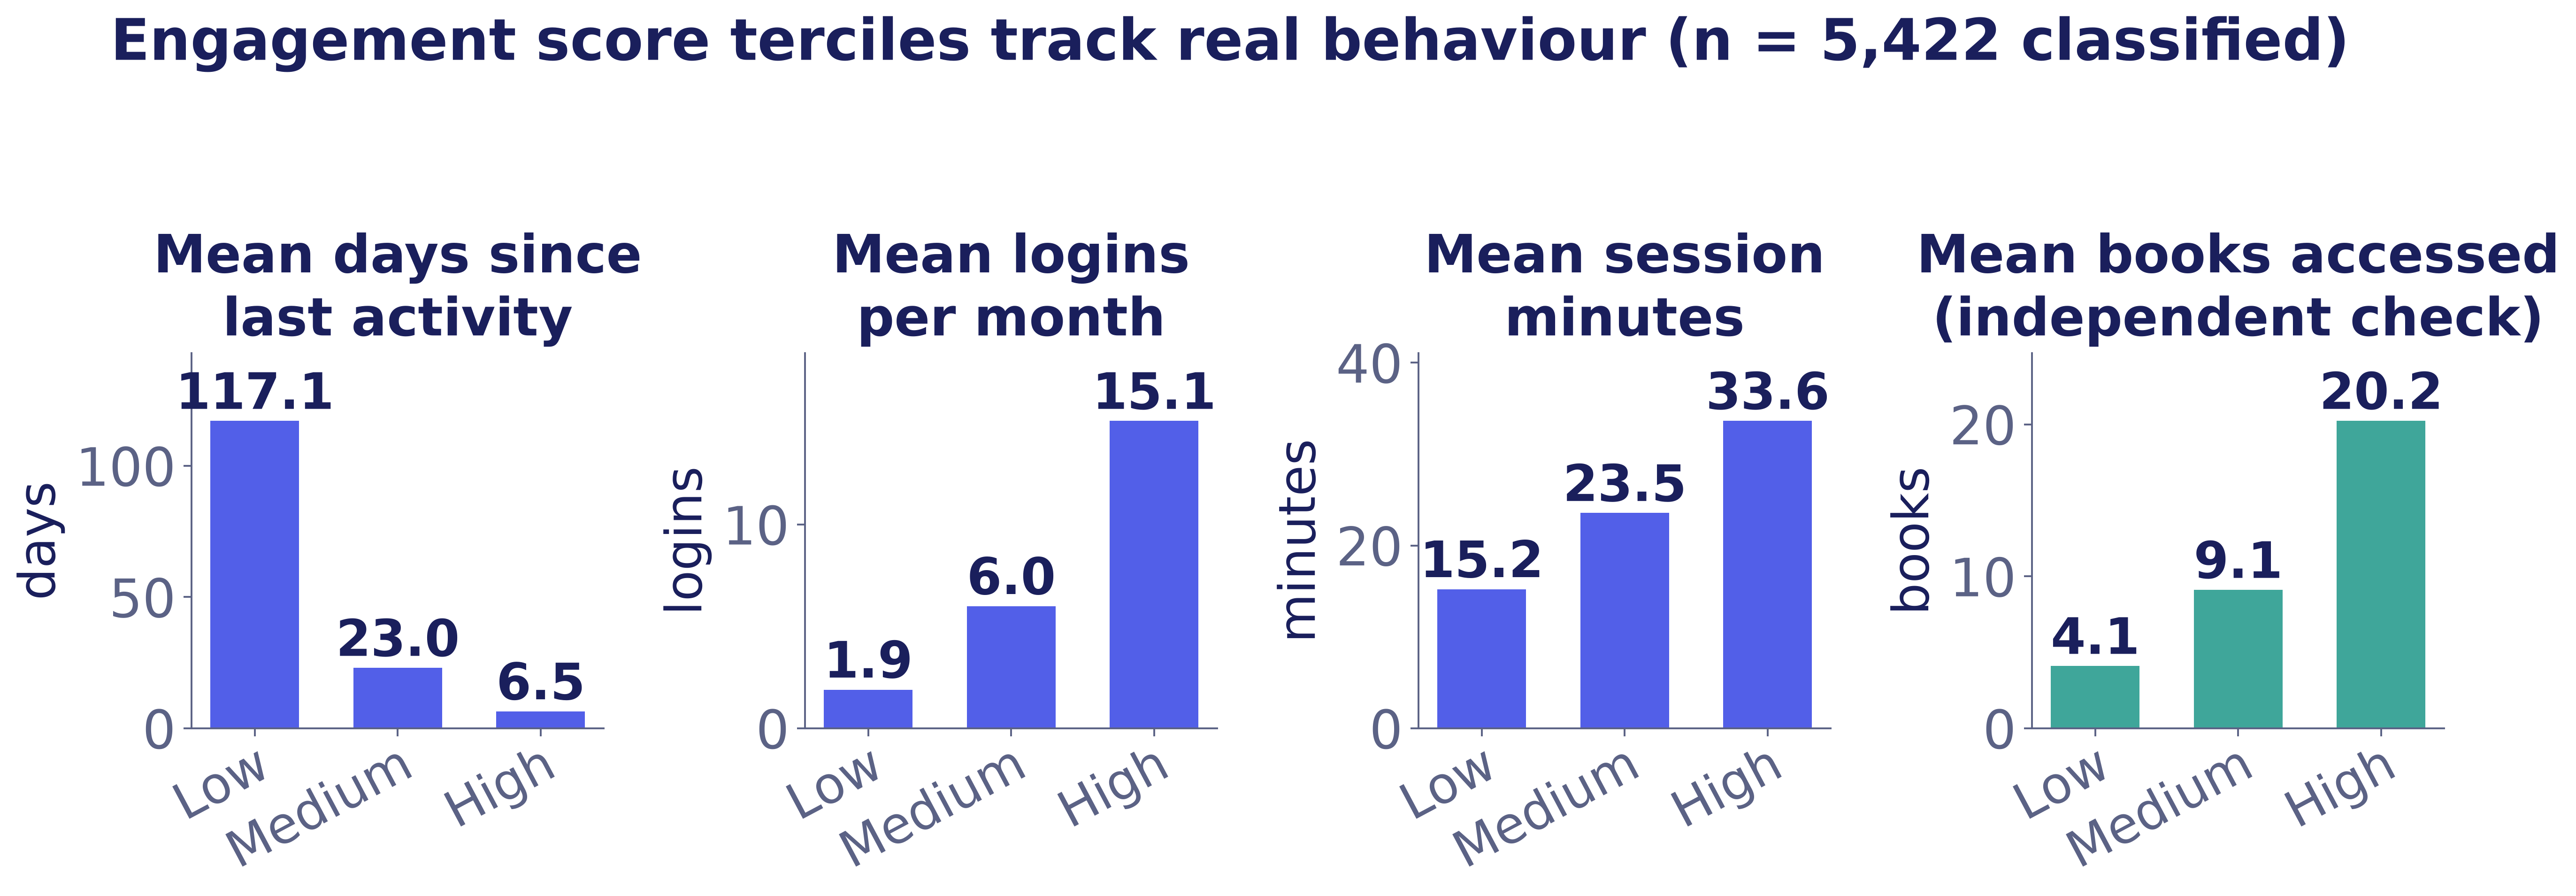
\includegraphics[width=0.80\linewidth]{figures/f2_tier_panels.png}
\captionof{figure}{Books accessed -- not a score input -- rise 4.1 $\rightarrow$ 9.1 $\rightarrow$ 20.2 across tiers: an independent check.}
\label{fig:tiers}

\vspace{0.4em}
\begin{minipage}{0.30\linewidth}
    \centering
    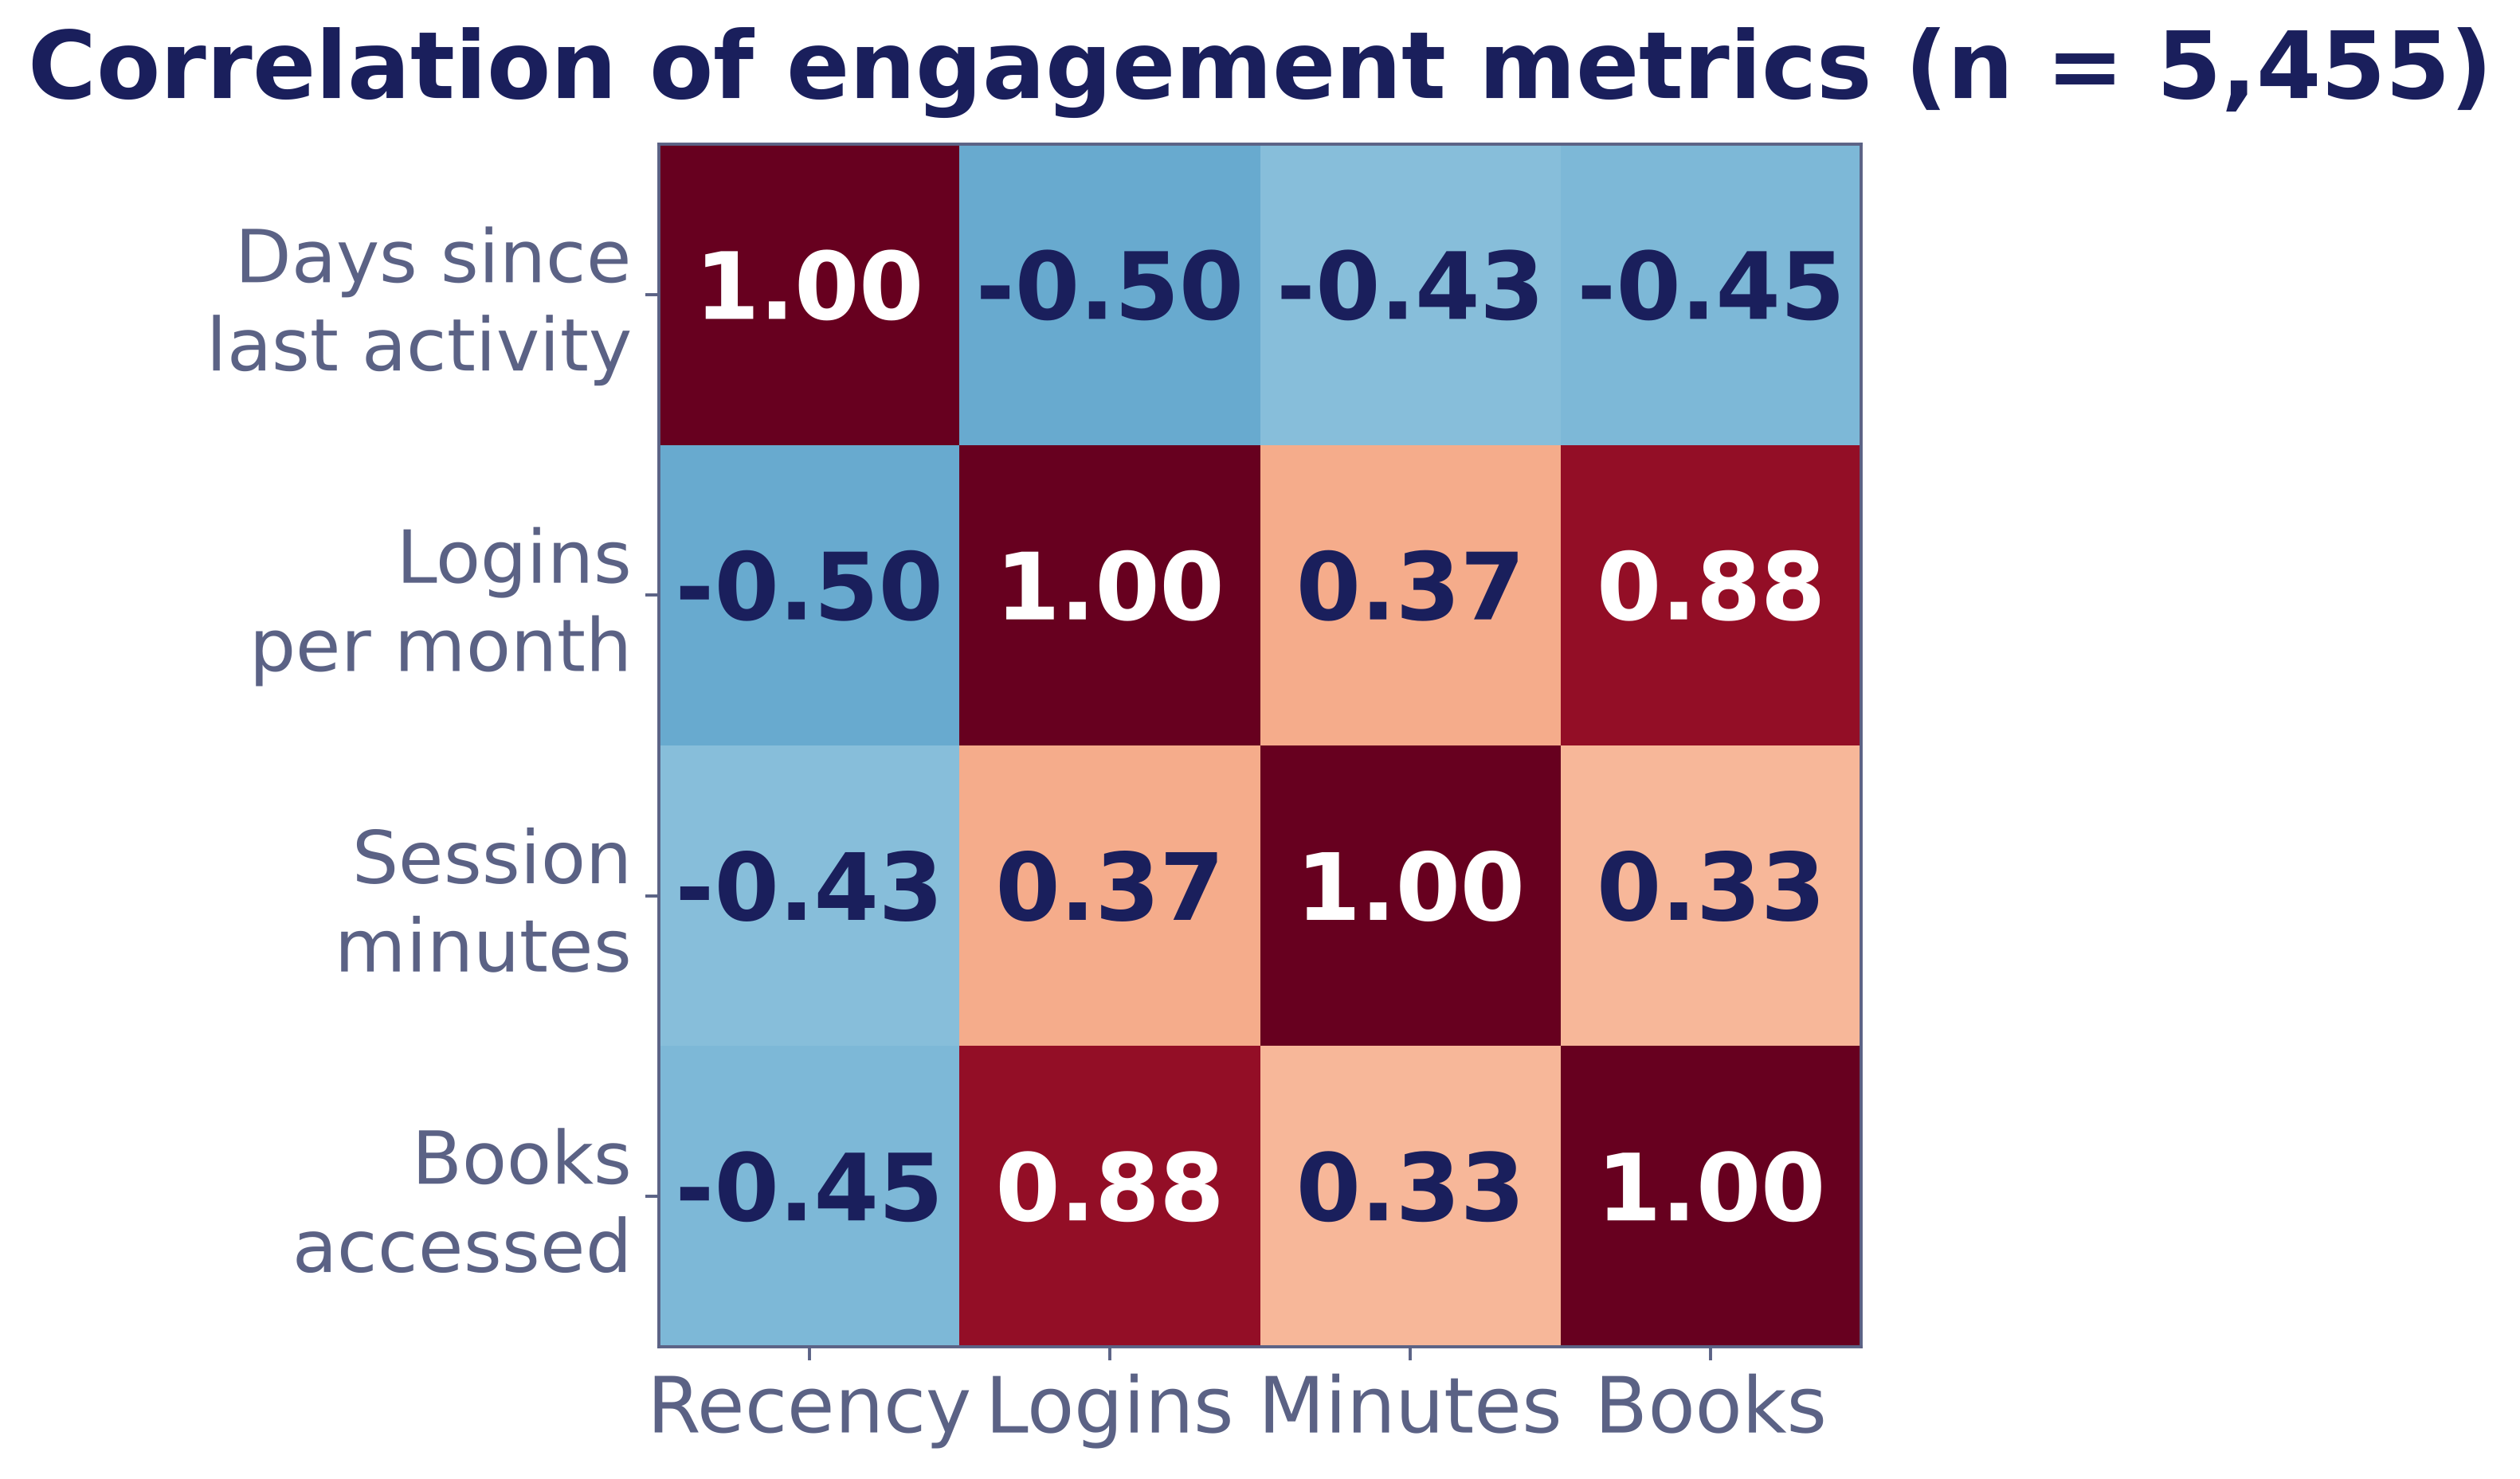
\includegraphics[width=\linewidth]{figures/f3_corr_heatmap.png}
    \captionof{figure}{$r = 0.88$: books excluded.}
    \label{fig:heat}
\end{minipage}

\end{block}

% ---------- 7. Tables ----------
\begin{block}{\textbf{Tables}}

\begin{center}
{\fontsize{15}{18}\selectfont
\captionof{table}{Status summary ($n = 5{,}455$)}
\label{tab:status}
\vspace{0.2em}

\renewcommand{\arraystretch}{1.0}
\setlength{\tabcolsep}{4pt}
\begin{tabular}{lccccc}
\toprule
\textbf{Status} & \textbf{n} & \textbf{\%} & \textbf{Median days} & \textbf{Mean logins} & \textbf{Mean books} \\
\midrule
Active & 3,001 & 55.3 & 5 & 11.7 & 16.1 \\
Inactive & 1,520 & 28.0 & 58 & 3.3 & 5.8 \\
\rowcolor{gray!15}
\textbf{Churned} & \textbf{901} & \textbf{16.6} & \textbf{152} & \textbf{1.5} & \textbf{3.6} \\
Unclassified & 33 & -- & -- & 9.9 & 13.1 \\
\bottomrule
\end{tabular}}
\end{center}

\end{block}

% ---------- 8. Insights & Interpretation ----------
\begin{block}{\textbf{Insights \& Interpretation}}
\begin{itemize}
\justifying
    \item \textbf{Churned subscribers log in far less}: 11.7 vs 1.5 logins a month, and the median gap since last activity is 5 / 58 / 152 days.
    \item \textbf{Books accessed rise by tier} (4.1 / 9.1 / 20.2) although books are \emph{not} a score input -- the score tracks real behaviour.
    \item \textbf{High-value vs Churned demographics are small} (T3, merged here): spend \$94.1 vs \$83.5 ($d = 0.33$), income \$99.8k vs \$90.3k (0.23), children 2.2 vs 1.7 (0.22), age 62.2 vs 63.8 ($-0.20$) -- all small, associations only, not causes.
    \item \textbf{Genre and tenure do not separate the groups}, and tier and status agree partly by construction because recency drives both.
    \item \textbf{Eleven Active subscribers sit in the Low tier} -- an early-warning watchlist.
\end{itemize}
\end{block}

% ---------- 9. Recommendations ----------
\begin{alertblock}{\textbf{Recommendations}}
\begin{itemize}
\justifying
    \item \emph{Active} -- \textbf{retain}: personalised recommendations, and monitor the 11 Low-tier Active subscribers.
    \item \emph{Inactive} -- \textbf{win back before day 90}: nudge near day 30 with personalised book picks and new releases.
    \item \emph{Churned} -- \textbf{win-back campaign} with relevant timing and segment-specific offers, not a blanket discount.
\end{itemize}
\end{alertblock}

% ---------- 10. Conclusion ----------
\begin{alertblock}{\textbf{Conclusion}}
\begin{itemize}
\justifying
    \item Declining logins and rising recency -- not demographics -- separate engagement groups; the score and status rules are reproducible.
    \item Limits: the study shows \emph{who} leaves and \emph{when}, not \emph{why}; associations only; status is recency-based; the data is synthetic.
    \item Next: pilot the three strategies on real data with cancellation dates.
\end{itemize}
\end{alertblock}

% ---------- References ----------
\begin{block}{\textbf{References}}
\vspace{-1em}
\fontsize{14}{17}\selectfont
\begin{multicols}{2}
\begin{thebibliography}{1}
\justifying
\setlength{\itemsep}{0pt}\setlength{\parskip}{0pt}
\bibitem{coussement2008}
K.~Coussement and D.~Van den Poel, ``Churn prediction in subscription services: An application of support vector machines,'' \emph{Expert Syst.\ Appl.}, 34(1):313--327, 2008.

\bibitem{bolton1999}
R.~N.~Bolton and K.~N.~Lemon, ``A dynamic model of customers' usage of services: Usage as an antecedent and consequence of satisfaction,'' \emph{J.~Mark.~Res.}, 36(2):171--186, 1999.

\bibitem{godinho2020}
M.~Godinho de Matos, P.~Ferreira, ``The effect of binge-watching on the subscription of video on demand: Results from randomized experiments,'' \emph{ISR}, 31(4):1337--1360, 2020.

\bibitem{rani2023}
M.~Rani, ``Understanding and managing customer churning in the SVOD industry,'' Master's thesis, UCP, 2023.

\bibitem{vuorinen2024}
P.~T.~E.~Vuorinen, B.~W.~Tatler, and F.~Keller, ``Tracking e-reading behavior: Uncovering the effects of task context, electronic experience, and motivation,'' \emph{Front.~Educ.}, 8:1302701, 2024.

\bibitem{gomezuribe2016}
C.~A.~Gomez-Uribe and N.~Hunt, ``The Netflix recommender system: Algorithms, business value, and innovation,'' \emph{ACM Trans.~Manag.~Inf.~Syst.}, 6(4):13:1--13:19, 2016.

\bibitem{thomas2004}
J.~S.~Thomas, R.~C.~Blattberg, and E.~J.~Fox, ``Recapturing lost customers,'' \emph{J.~Mark.~Res.}, 41(1):31--45, 2004.

\bibitem{ascarza2018}
E.~Ascarza, ``Retention futility: Targeting high-risk customers might be ineffective,'' \emph{J.~Mark.~Res.}, 55(1):80--98, 2018.

\end{thebibliography}
\end{multicols}

\end{block}

\end{column}
\separatorcolumn



\end{columns}
\end{frame}

\end{document}
